\section{Future Work}
\label{futurework}

Attractive innovation that could be added into the already existing eclipse plugin are the follow:

- Intent dependencies and options.
	Adding this feature, which will consist on adding some instructions or guide into the plugin interface as description next to the intent, or while the users hovers on top of the selected intent options. To understand better the following option. 

\begin{figure}[H]
\label{codegeneratorview}
  \centering
    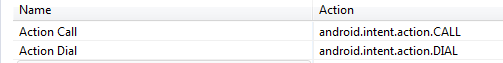
\includegraphics[width=\textwidth]{intentBefore}
  \caption{Future Work 1.0}
\end{figure}

	As we can see right now their is a lack of information which makes harder to decide for new developers/programmers which intent is the more appropriate selection for their needs.

- Creating constants and variables
	To streamline for creating a better and faster experience while using this plugin, there is the need to create constants and variables when they are generated when inserting an intent.

- API level support, which implicates to be able to read which API level does the applications is build on top of, and insert an alternative if the current intent is not support it by current API level.
	